\documentclass[11pt]{article}

\usepackage{../algebra}

\begin{document}

\coverpage{3}

% hw problem 1 -----------------------------------------------------------------

\begin{exercise}{48}{29}
    \problem{
        Let $G$ be a finite, nonempty set with an operation $\ast$ such that: \\
        \indent 1. $G$ is closed under $\ast$ \\
        \indent 2. $\ast$ is associative \\
        \indent 3. Given $a,b,c \in G$ with $a \ast b = a \ast c$, then $b = c$ \\
        \indent 4. Given $a,b,c \in G$ with $b \ast a = c \ast a$, then $b = c$ \\
        Prove that $G$ must be a group under $\ast$.
    }
    \proof{
        To prove that $(G, \ast)$ is a group, we must show that $G$ contains an identity element and an inverse for each element.
        Let's begin with the identity element.
        We must find an element $e \in G$ such that $x \ast e = e \ast x = x$ for all $x \in G$.
        Let $|G| = n < + \infty$ and fix an element $g \in G$ and consider $g, g^2, g^3, ..., g^{n+1}$.
        Since $G$ is closed under $\ast$, every $g^k$ is an element of $G$, yet $G$ has only $n$ elements so we must have $g^i = g^j$ for some $1 \leq i < j \leq n+1$. \parspace
        Now let $l = j-i > 0$ (which means $j = l+i = i+l$) and we can say that $g^j = g^{l+i} = g^l \ast g^i$ and $g^j = g^{i+l} = g^i \ast g^l$.
        But then $g^j = g^i$ so we have $g^i = g^i \ast g^l = g^l \ast g^i$.
        Letting $g^i = \bar{g}$ and $g^l = \bar{e}$ (both elements of $G$ by closure under $\ast$) gives us $\bar{g} = \bar{g} \ast \bar{e} = \bar{e} \ast \bar{g}$ for the specific element $\bar{g} \in G$. \parspace
        We now show that $\bar{e}$ is an identity element for every element of $G$.
        Fix any $x \in G$, then $\bar{g} \ast x = \bar{g} \ast \bar{e} \ast x$ since $\bar{g} = \bar{g} \ast \bar{e}$.
        But then property 3 says that $x = \bar{e} \ast x$.
        Further, $x \ast \bar{g} = x \ast \bar{e} \ast \bar{g}$ since $\bar{e} \ast \bar{g} = \bar{g}$ and then property 4 allows us to say that $x \ast \bar{e} = x$.
        So we have just shown that $x \ast \bar{e} = \bar{e} \ast x = x$ for an arbitrary $x \in G$.
        In other words, $\bar{e}$ is an identity element for $G$. \parspace
        Now we must show an inverse element exists for every element of $G$: that there exists some element $g' \in G$ such that $g \ast g' = g' \ast g = \bar{e}$.
        To do this, we take $g$ and $g^l = \bar{e}$ as before.
        Pick $g' = g^{l-1} \in G$ then $g \ast g' = g \ast g^{l-1} = g^{1+l-1} = g^{l+1-1} = g^l = \bar{e}$ and $g' \ast g = g^{l-1} \ast g = g^{l-1+1} = g^l = \bar{e}$ as desired.
        Since we chose $g$ arbirarily, we have just shown every element has an inverse in $G$. \parspace
        So we have showed that an identity exists in $G$ and each element has an inverse so $G$ satisfies the conditions of a group.
    }
\end{exercise}

% hw problem 2 -----------------------------------------------------------------

\begin{exercise}{54}{3}
    \problem{
        Let $S_3$ be the symmetric group of degree 3.
        Find all the subgroups of $S_3$.
    }
    \proof{
        First note that we always have the trivial subgroups $\{ id \}$ and $S_3$.
        We must now find the remaining subgroups of $S_3$.
        Note that $|S_3| = 3! = 6$ and for any subgroup $H \leq S_3$, we must have $id \in H$.
        This leaves us only 5 options to include in a subgroup $H$.
        If we choose one of the elements $(1 2), (2 3), (1 3)$ to accompany $id$ then we have a subgroup for each of those elements is it's own inverse.
        So in addition to the trivial subgroups we also have $\{ id, (1 2) \}, \{ id, (2 3) \}, \{ id, (1 3) \}$. \parspace
        Note that the remaining elements we can choose to accompany $id$ are $(1 2 3) = (3 1 2) = (2 3 1)$ and $(1 3 2) = (2 1 3) = (3 2 1)$.
        Now suppose we choose one of $(1 2 3), (1 3 2)$ to accompany $id$.
        Then Figure \ref{fig:closure1} shows that the other must also be in the subgroup to satisfy closure.
        Also each of them applied 3 times to the themselves so we have inverses as well.
        Therefore $\{ id, (1 2 3), (1 3 2) \}$ constitutes a subgroup as well.

        \begin{figure}[h]
            \centering
            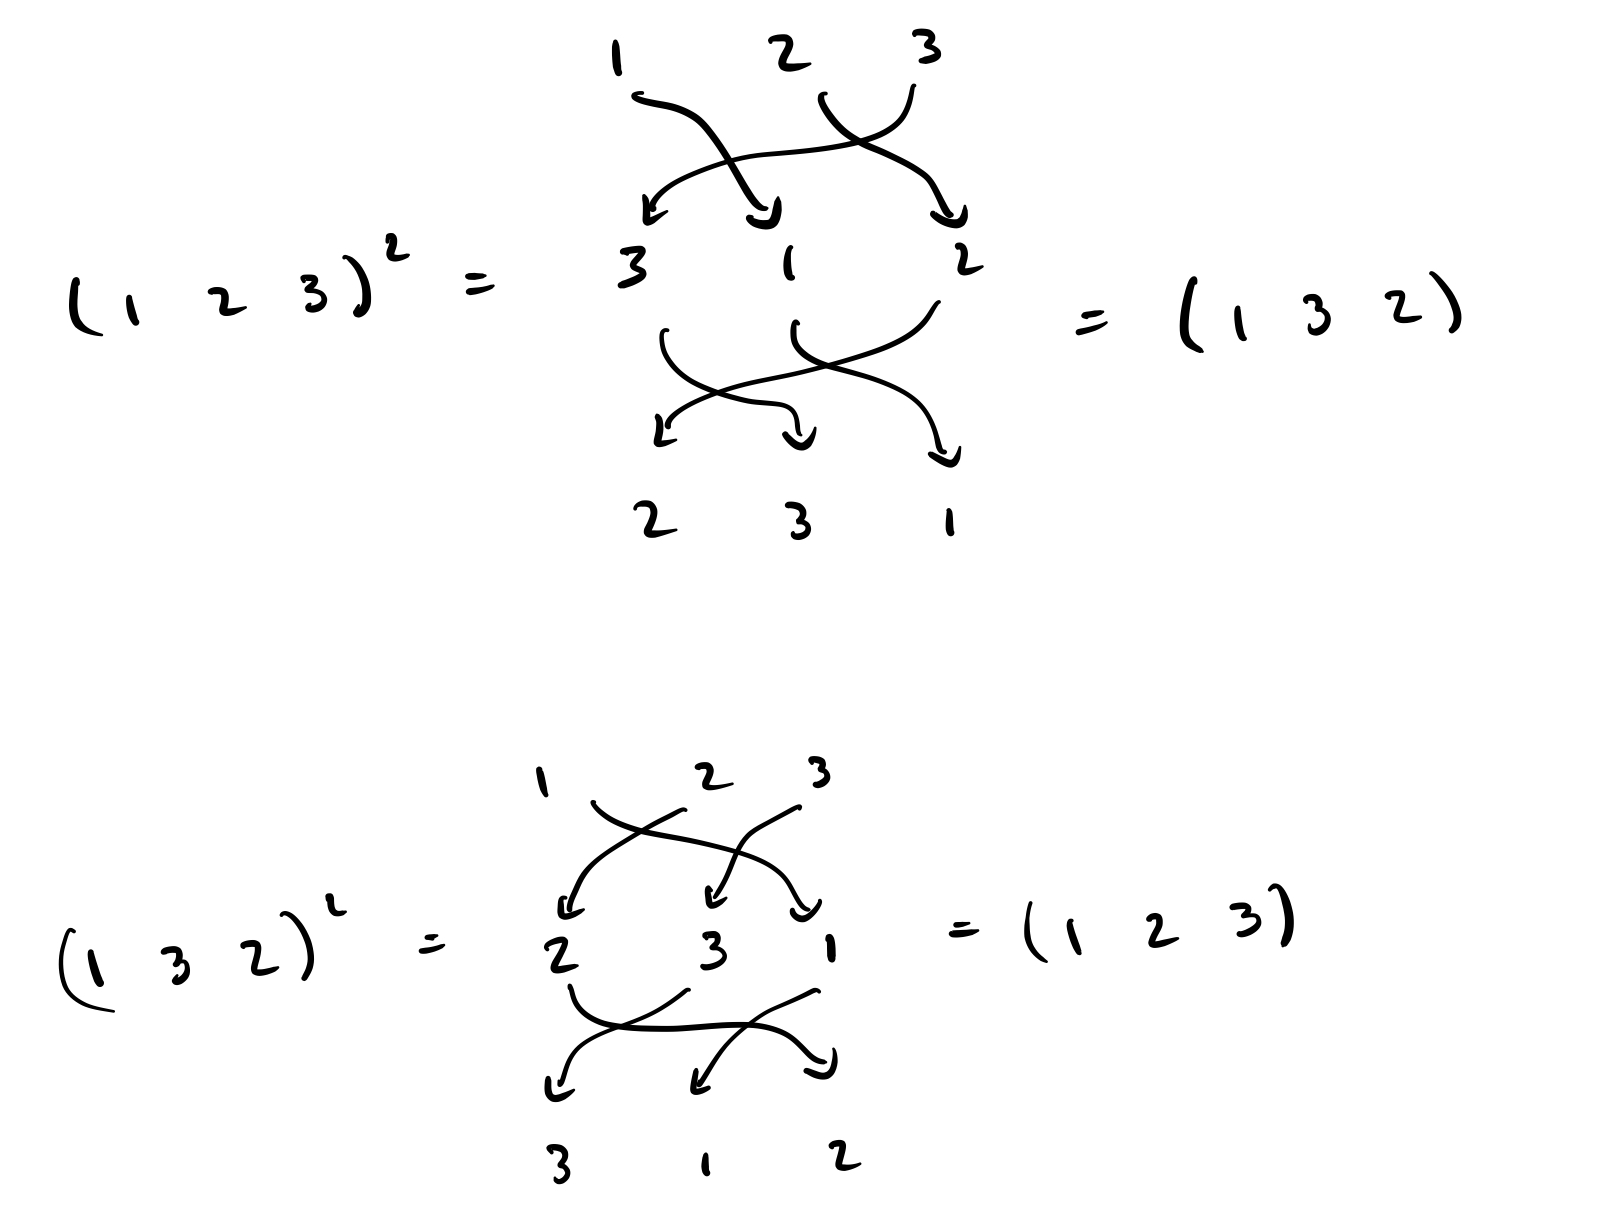
\includegraphics[width=0.5\textwidth]{img/closure1}
            \caption{Necessary closure for 3 cycles}
            \label{fig:closure1}
        \end{figure}

        \newpage
        We now show that we have listed all subgroups of $S_3$.
        We can deduce this from the requirement that a subgroup requires closure.
        Of the remaining combinations of elements we could choose to accompany $id$ in a subgroup, all of them require including the whole group.
        This is shown in Figures \ref{fig:closure2} and \ref{fig:closure3}.
        As an example pick elements $(1 2), (2 3)$ to accompany $id$.
        To satisfy closure, we must include $(1 2 3)$ (Figure \ref{fig:closure2}) but then we must include $(1 3 2)$ (Figure \ref{fig:closure1}) and then we must include $(1 3)$ (Figure \ref{fig:closure3}) which is the entire set.

        \begin{figure}[h]
            \centering
            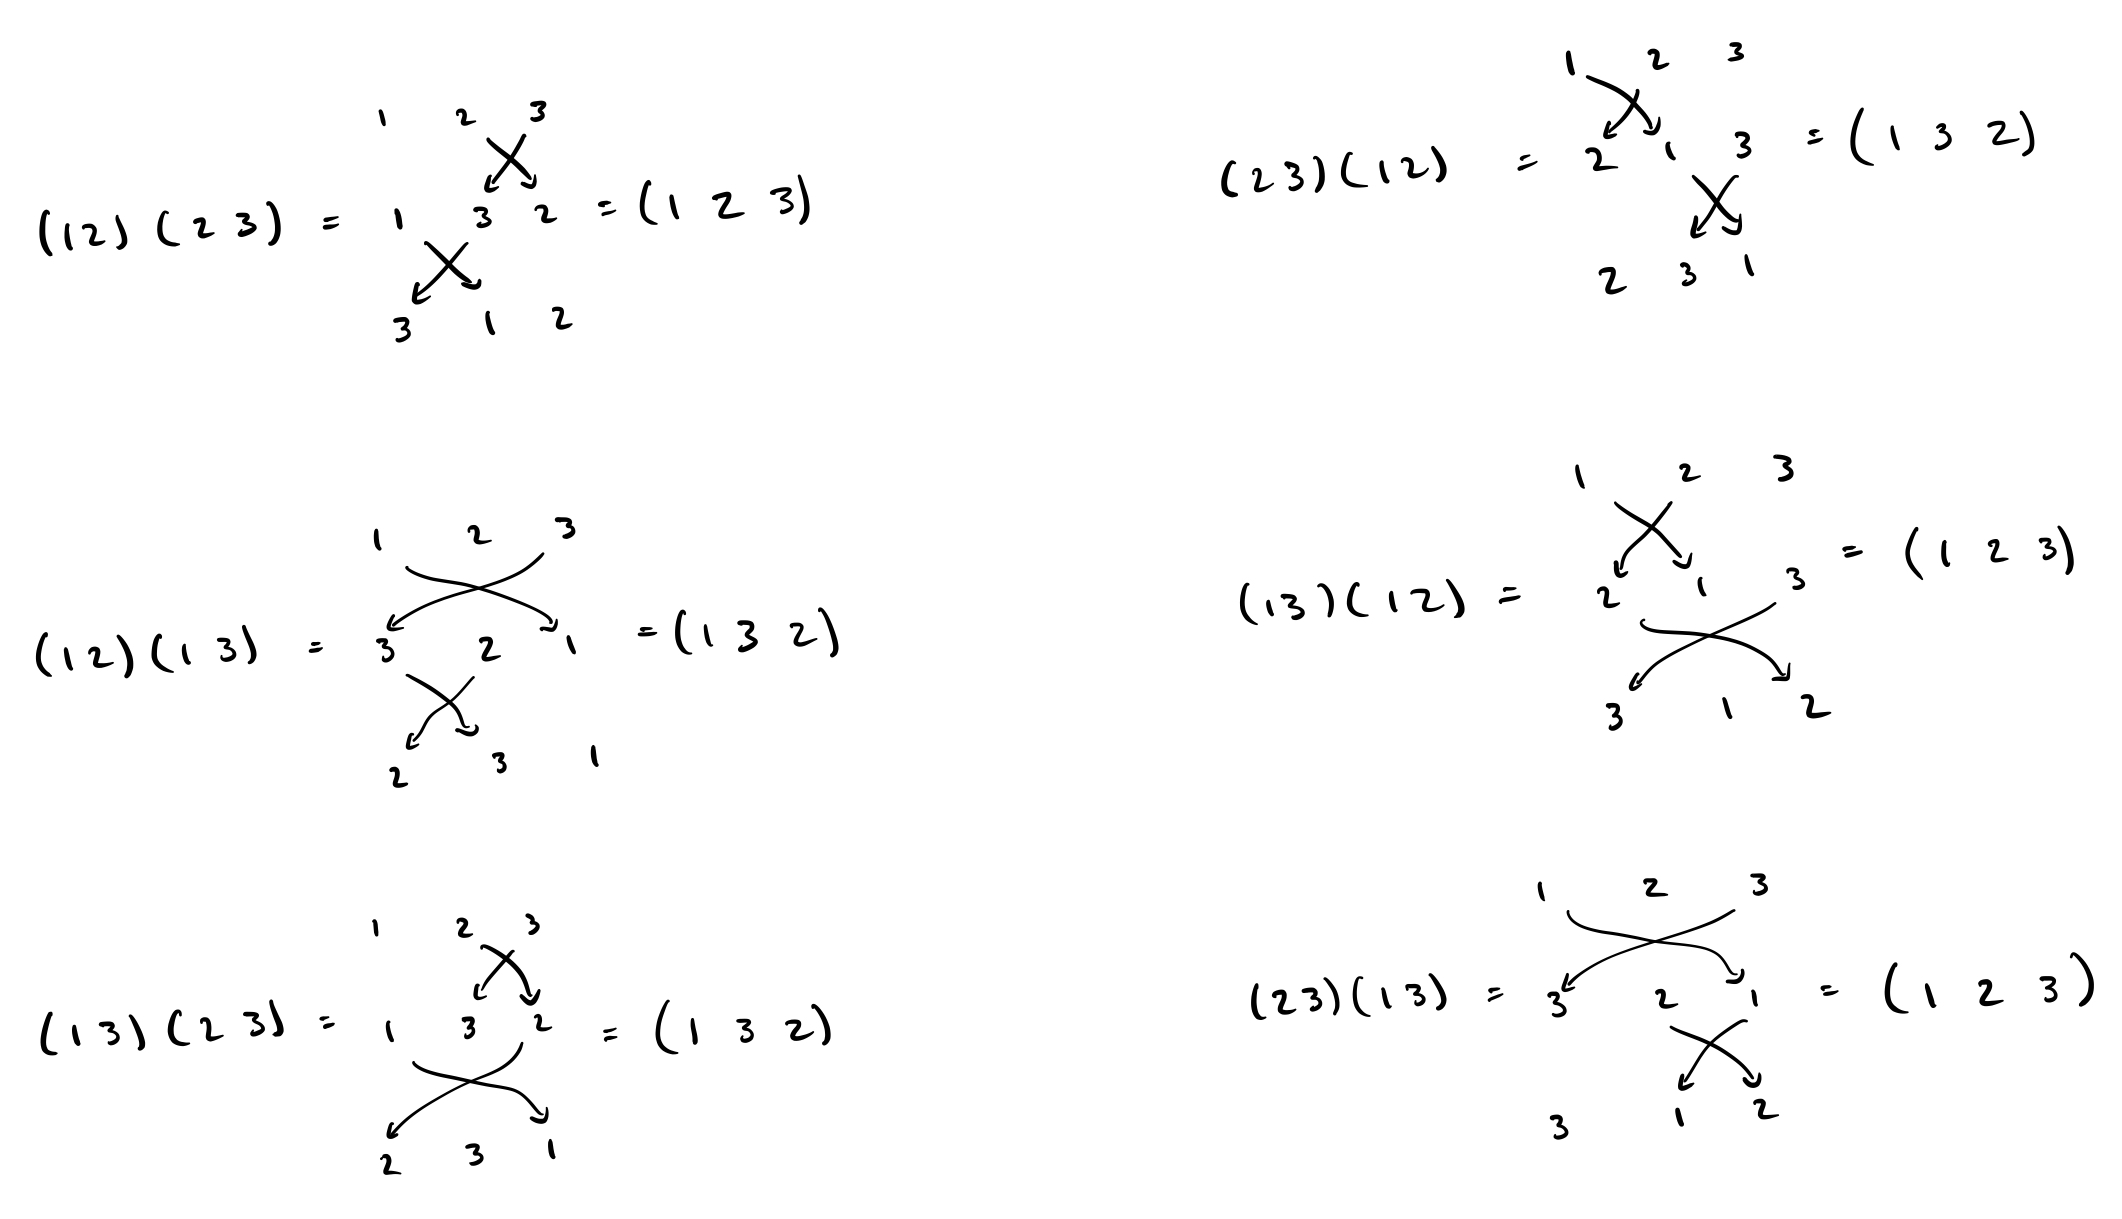
\includegraphics[width=0.75\textwidth]{img/closure2}
            \caption{Necessary closures}
            \label{fig:closure2}
        \end{figure}
        \begin{figure}[h]
            \centering
            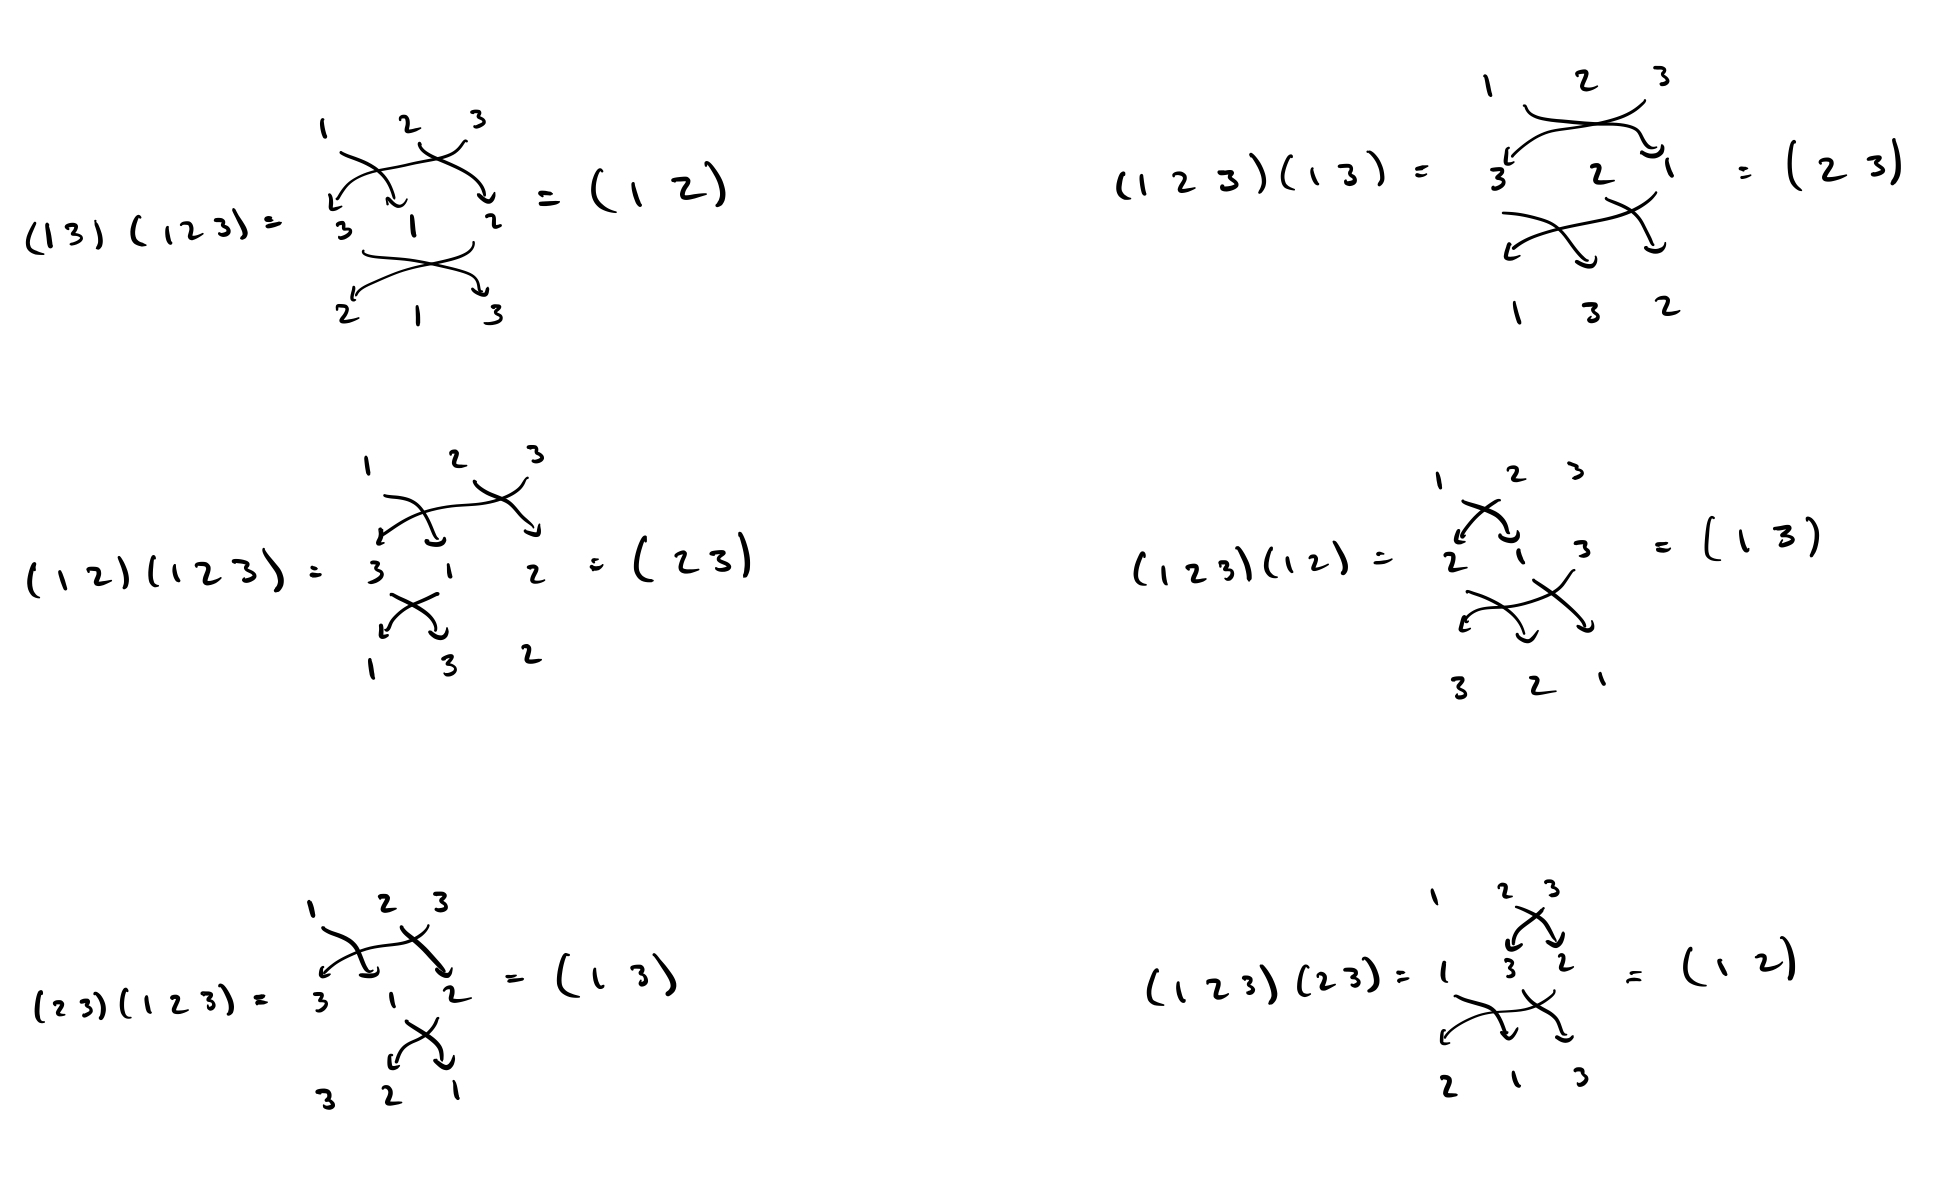
\includegraphics[width=0.75\textwidth]{img/closure3}
            \caption{Necessary closures}
            \label{fig:closure3}
        \end{figure}
    }
\end{exercise}

% hw problem 3 -----------------------------------------------------------------

\begin{exercise}{55}{12}
    \problem{
        Prove that a cyclic group is abelian.
    }
    \proof{
        Let's first introduce the definition of a cyclic group.
        A group $G$ is cyclic if there exists some $a \in G$ such every $x \in G$ is a power of $a$ ($x = a^j$ for some $j \in \Z$).
        Additionally, a group is abelian if $ab = ba$ for all $a,b \in G$. \parspace
        Suppose we have some cyclic group $G$.
        Since $G$ is cyclic, there is some $g \in G$ such that every $x \in G$ is of the form $x = g^j$ for some $j \in \Z$.
        Now take any $a,b \in G$ and note that $a = g^i$ and $b = g^k$ for some $i,k \in Z$.
        Then $ab = g^i g^k = g^{i+k} = g^{k+i} = g^k g^i = ba$ as desired.
        Therefore, every cyclic group is abelian.
    }
\end{exercise}

% hw problem 4 -----------------------------------------------------------------

\newpage
\section*{Heisenberg group problem}
    \problem{
        Recall the general linear group $\GL _3(\R)$ of $3 \times 3$ invertible matrices with real entries (taken with the matrix product).
        Verify that the following subset, called the Heisenberg group, is a subgroup of $\GL _3 (\R)$:
        $$ \H _3 (\R) :=
        \left\{
            \begin{bmatrix}
                1 & x & z \\
                0 & 1 & y \\
                0 & 0 & 1
            \end{bmatrix}
            \mid x,y,z \in \R
        \right\} $$
    }
    \proof{
        First we note that $\H _3 (\R)$ is a (nonempty) subset of $\GL _3 (\R)$ since $I_3 \in \H _3 (\R)$ and every matrix in $\H _3 (\R)$ has rank 3.
        Then since $\H _3 (\R) \subset \GL _3 (\R)$ we automatically inherit the associativity of matrix multiplication.
        So only two conditions remain for $\H _3 (\R)$ to be a subgroup: closure and the existence of an inverse in $\H _3 (\R)$.
        The previous two conditions imply $I_3 \in \H _3 (\R)$ but this was also verified by inspection. \parspace
        Let's first prove closure.
        Pick $A, A' \in \H _3 (\R)$ and compute
        $$ A A' =
        \begin{bmatrix}
            1 & x & z \\
            0 & 1 & y \\
            0 & 0 & 1
        \end{bmatrix}
        \begin{bmatrix}
            1 & x' & z' \\
            0 & 1 & y' \\
            0 & 0 & 1
        \end{bmatrix}
        =
        \begin{bmatrix}
            1 & x'+x & z'+xy'+z \\
            0 & 1 & y'+y \\
            0 & 0 & 1
        \end{bmatrix}
        =
        \begin{bmatrix}
            1 & \bar{x} & \bar{z} \\
            0 & 1 & \bar{y} \\
            0 & 0 & 1
        \end{bmatrix}
        \in \H _3 (\R)
        $$
        where $\bar{x}, \bar{y}, \bar{z} \in \R$ by the closure of $\R$ under addition and multiplication.
        So $\H _3 (\R)$ is closed under matrix multiplication.
        We must now show that for every $A \in \H _3 (\R)$ we also have $B \in \H _3 (\R)$ such that $AB = BA = I_3$.
        For $A$, choose
        $$ B =
        \begin{bmatrix}
            1 & -x & xy-z \\
            0 & 1 & -y \\
            0 & 0 & 1
        \end{bmatrix}$$
        Certainly $B$ is in the set $\H _3 (\R)$ and we have
        $$AB =
        \begin{bmatrix}
            1 & x & z \\
            0 & 1 & y \\
            0 & 0 & 1
        \end{bmatrix}
        \begin{bmatrix}
            1 & -x & xy-z \\
            0 & 1 & -y \\
            0 & 0 & 1
        \end{bmatrix}
        =
        \begin{bmatrix}
            1 & 0 & 0 \\
            0 & 1 & 0 \\
            0 & 0 & 1
        \end{bmatrix}
        =
        \begin{bmatrix}
            1 & -x & xy-z \\
            0 & 1 & -y \\
            0 & 0 & 1
        \end{bmatrix}
        \begin{bmatrix}
            1 & x & z \\
            0 & 1 & y \\
            0 & 0 & 1
        \end{bmatrix}
        = BA
        $$
        So we have checked that $\H _3 (\R)$ is closed under matrix multiplication and every element has an inverse in the subset so $\H _3 (\R)$ is a subgroup of $\GL _3 (\R)$.
    }

% hw problem 5 -----------------------------------------------------------------

\newpage
\section*{Cube subgroups problem}
    \problem{
        Recall the group $Sym(Q)$ of the rigid symmetries of the cube $Q := [-1,1]^3$ in $\R ^3$.
        Describe in words/pictures the following: \\
        \indent a subgroup of order 4 \\
        \indent a subgroup of order 12 \\
        \indent a subgroup of order 3 \\
        \indent a subgroup of order 6 \\
        \indent a subgroup of order 8
    }
    \proof{
        For the purposes of this problem, we label the initial faces of the cube as you would a die (with side one facing us and side 6 opposite and so on).
        \begin{figure}[h]
            \centering
            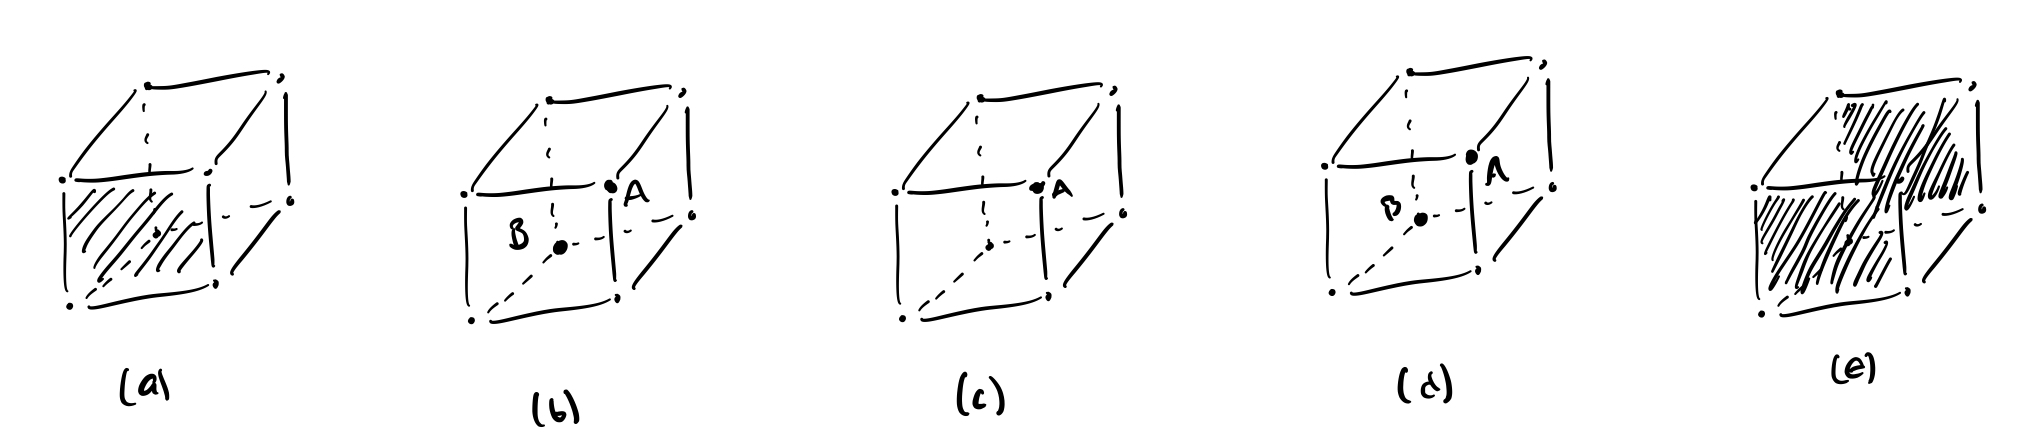
\includegraphics[width=0.9\textwidth]{img/cubegroups}
            \caption{Subgroups of a cube}
            \label{fig:cubegroups}
        \end{figure}

        \noindent
        {\bf Order 4:}
        We can make subgroup of order 4 by keeping all rigid symmetries of $Q$ that keep us looking at the same face.
        In Figure \ref{fig:cubegroups}a we shaded in this face.
        The subgroup is any symmetric rotation about the x axis, of which there are 4. \parspace
        {\bf Order 12:} I found and order 12 subgroup to be the most difficult to find.
        Here is what I have landed on: any rigid symmetry that preserves $A$'s position in Figure \ref{fig:cubegroups}b and a rotation by $\pi$ about the z axis.
        The next part says that preserving $A$ is a group of order 3 and then we get four distinct subgroups from the points that could end up in $A$'s location (these are $A$ and each of the points across the diagonal of a {\it square} touching $A$).
        Then the subgroup is of order 12. \parspace
        {\bf Order 3:} A subgroup of order 3 can be found by requiring that the vertex labed $A$ in Figure \ref{fig:cubegroups}c stays in the same location.
        This allows us three actions, synonomous with spinning the cube about $A$ and the point diagonally through the cube from $A$. \parspace
        {\bf Order 6:} An order 6 subgroup is pretty similar to the order 3 subgroup we just discussed.
        Instead of requiring that $A$ stays in the same location, we say that $A$ and $B$ in Figure \ref{fig:cubegroups}d must remain on the diagonal they begin on.
        This gives the three actions when $A$ is stationary and another three actions when we flip $A$ and $B$ (which can be done by a rotation by $\pi$ about z axis and then a rotation by $\pi /2$ about x axis). \parspace
        {\bf Order 8:} For a subgroup of order 8, we require that we look at one of the two shaded faces shown in Figure \ref{fig:cubegroups}e.
        This gives us four actions while looking at face 1 and another four while looking at face 6. \parspace
    }

\end{document}
